\documentclass[UTF8]{article}
\usepackage{amsmath}
\usepackage{graphicx}
\usepackage{amssymb}

\title{Machine Learning Note}
\date{}
\begin{document}

\maketitle
\tableofcontents

\section{Lecture 1}

\subsection{What is Machine Learning?}
Two definitions of Machine Learning are offered. 

Arthur Samuel described it as: ``the field of study that gives computers the ability to learn without being explicitly programmed." This is an older, informal definition.

Tom Mitchell provides a more modern definition: ``A computer program is said to learn from experience E with respect to some class of tasks T and performance measure P, if its performance at tasks in T, as measured by P, improves with experience E."

In general, any machine learning problem can be assigned to one of two broad classifications: Supervised learning and Unsupervised learning.

\paragraph{Example}Playing checkers.

E = the experience of playing many games of checkers.

T = the task of playing checkers.

P = the probability that the program will win the next game.

\subsection{Supervised Learning}

In supervised learning, we are given a data set and already know what our correct output should look like, having the idea that there is a relationship between the input and the output.

Supervised learning problems are categorized into ``regression" and ``classification" problems. In a regression problem, we are trying to predict results within a continuous output, meaning that we are trying to map input variables to some continuous function. In a classification problem, we are instead trying to predict results in a discrete output. In other words, we are trying to map input variables into discrete categories.

\paragraph{Example 1}  

Given data about the size of houses on the real estate market, try to predict their price. Price as a function of size is a continuous output, so this is a regression problem.

We could turn this example into a classification problem by instead making our output about whether the house ``sells for more or less than the asking price." Here we are classifying the houses based on price into two discrete categories.

\paragraph{Example 2}  

(a) Regression - Given a picture of a person, we have to predict their age on the basis of the given picture

(b) Classification - Given a patient with a tumor, we have to predict whether the tumor is malignant or benign.

\subsection{Unsupervised Learning}

Unsupervised learning allows us to approach problems with little or no idea what our results should look like. We can derive structure from data where we don't necessarily know the effect of the variables.

We can derive this structure by clustering the data based on relationships among the variables in the data.

With unsupervised learning there is no feedback based on the prediction results.

\paragraph{Example}

Clustering: Take a collection of 1,000,000 different genes, and find a way to automatically group these genes into groups that are somehow similar or related by different variables, such as lifespan, location, roles, and so on.

Non-clustering: The ``Cocktail Party Algorithm", allows you to find structure in a chaotic environment. (i.e. identifying individual voices and music from a mesh of sounds at a cocktail party).

\section{Lecture 2}

\subsection{Model Representation}

To establish notation for future use, we will use $x^{(i)}$ to denote the ``input'' variables (living area in this example), also called input features, and $y^{(i)}$ to denote the ``output'' or target variable that we are trying to predict (price). A pair $(x^{(i)},y^{(i)})$ is called a training example, and the dataset that we'll be using to learn - a list of m training examples $(x^{(i)},y^{(i)}); i=1,...,m$ - is called a training set. Note that the superscript $(i)$ in the notation is simply an index into the training set, and has nothing to do with exponentiation. We will also use $X$ to denote the space of input values, and $Y$ to denote the space of output values.

To describe the supervised learning problem slightly more formally, our goal is, given a training set, to learn a function $h$: $X \to Y$ so that $h(x)$ is a ``good'' predictor for the corresponding value of $y$. For historical reasons, this function $h$ is called a hypothesis. Seen pictorially, the process is therefore like this:

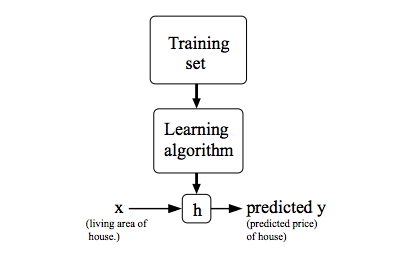
\includegraphics[width = .8\textwidth]{NotePics/2_1_1.png}

When the target variable that we are trying to predict is continuous, such as in our housing example, we call the learning problem a regression problem. When $y$ can take on only a small number of discrete values (such as if, given the living area, we wanted to predict if a dwelling is a house or an apartment, say), we call it a classification problem.

\subsection{Cost Function}

We can measure the accuracy of our hypothesis function by using a cost function. This takes an average difference (actually a fancier version of an average) of all the results of the hypothesis with inputs from $x$'s and the actual output $y$'s.

\[ J(\theta_0,\theta_1)=\frac{1}{2m}\sum_{i=1}^{m}(\hat{y_i} - y_i)^2=\frac{1}{2m}\sum_{i=1}^{m}(h_\theta{(x_i)} - {y_i})^2 \]

To break it apart, it is $\frac{1}{2}\bar{x}$ where $\bar{x}$ is the mean of the squares of $h_\theta(x_i) - y_i$ , or the difference between the predicted value and the actual value.

This function is otherwise called the ``Squared error function'', or ``Mean squared error". The mean is halved ($\frac{1}{2}$) as a convenience for the computation of the gradient descent, as the derivative term of the square function will cancel out the $\frac{1}{2}$ term. The following image summarizes what the cost function does:

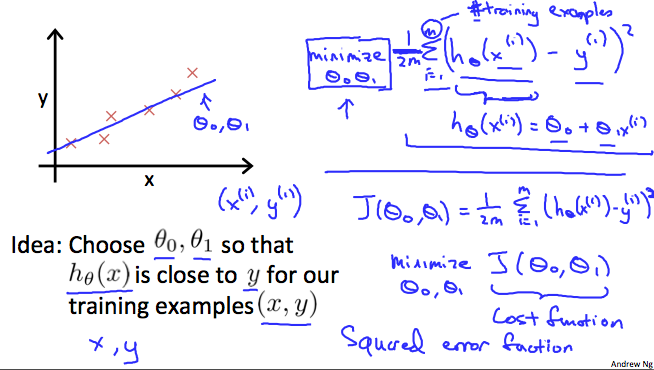
\includegraphics[width = .8\textwidth]{NotePics/2_2_1.png}

\subsubsection{Cost Function - Intuition I}

If we try to think of it in visual terms, our training data set is scattered on the $x-y$ plane. We are trying to make a straight line (defined by $h_\theta(x)$) which passes through these scattered data points.

Our objective is to get the best possible line. The best possible line will be such so that the average squared vertical distances of the scattered points from the line will be the least. Ideally, the line should pass through all the points of our training data set. In such a case, the value of $J(\theta_0,\theta_1)$ will be 0. The following example shows the ideal situation where we have a cost function of 0.

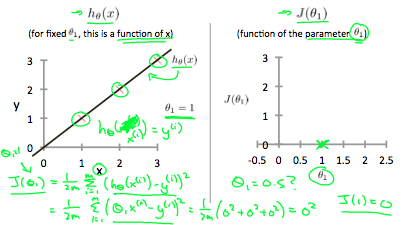
\includegraphics[width = .8\textwidth]{NotePics/2_2_1_1.png}

When $\theta_1=1$, we get a slope of 1 which goes through every single data point in our model. Conversely, when $\theta_1=0.5$, we see the vertical distance from our fit to the data points increase.

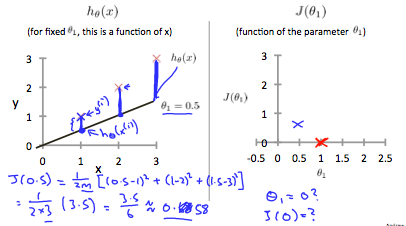
\includegraphics[width = .8\textwidth]{NotePics/2_2_1_2.png}

This increases our cost function to 0.58. Plotting several other points yields to the following graph:

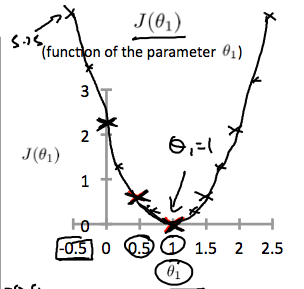
\includegraphics[width = .8\textwidth]{NotePics/2_2_1_3.png}

Thus as a goal, we should try to minimize the cost function. In this case, $\theta_1=1$ is our global minimum.

\subsubsection{Cost Function - Intuition II}

A contour plot is a graph that contains many contour lines. A contour line of a two variable function has a constant value at all points of the same line. An example of such a graph is the one to the right below.

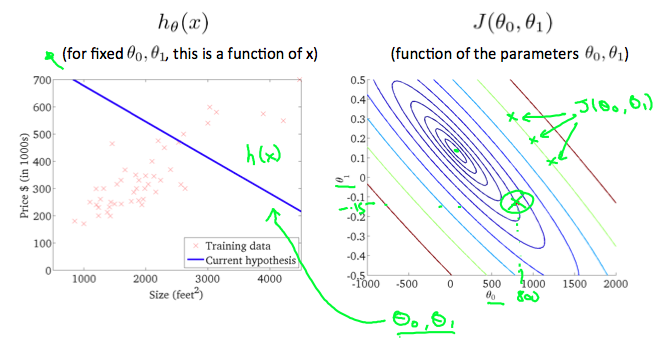
\includegraphics[width = .8\textwidth]{NotePics/2_2_2_1.png}

Taking any color and going along the `circle', one would expect to get the same value of the cost function. For example, the three green points found on the green line above have the same value for $J(\theta_0,\theta_1)$ and as a result, they are found along the same line. The circled x displays the value of the cost function for the graph on the left when $\theta_0 = 800$ and $\theta_1= -0.15$. Taking another $h(x)$ and plotting its contour plot, one gets the following graphs:

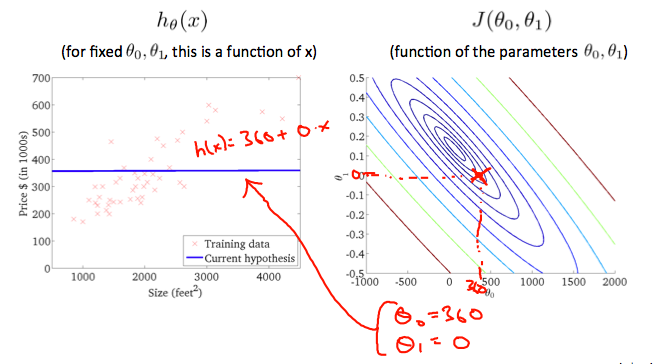
\includegraphics[width = .8\textwidth]{NotePics/2_2_2_2.png}

When $\theta_0 = 360$ and $\theta_1 = 0$, the value of $J(\theta_0,\theta_1)$ in the contour plot gets closer to the center thus reducing the cost function error. Now giving our hypothesis function a slightly positive slope results in a better fit of the data.

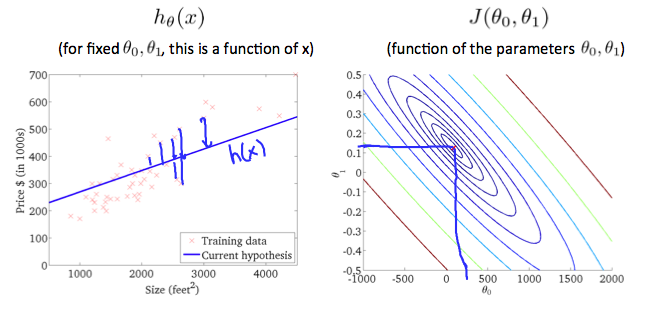
\includegraphics[width = .8\textwidth]{NotePics/2_2_2_3.png}

The graph above minimizes the cost function as much as possible and consequently, the result of $\theta_1$ and $\theta_0$ tend to be around 0.12 and 250 respectively. Plotting those values on our graph to the right seems to put our point in the center of the inner most `circle'.

\subsection{Gradient Descent}

So we have our hypothesis function and we have a way of measuring how well it fits into the data. Now we need to estimate the parameters in the hypothesis function. That's where gradient descent comes in.

Imagine that we graph our hypothesis function based on its fields $\theta_0$ and $\theta_1$ (actually we are graphing the cost function as a function of the parameter estimates). We are not graphing $x$ and $y$ itself, but the parameter range of our hypothesis function and the cost resulting from selecting a particular set of parameters.

We put $\theta_0$ on the $x$ axis and $\theta_1$ on the $y$ axis, with the cost function on the vertical $z$ axis. The points on our graph will be the result of the cost function using our hypothesis with those specific theta parameters. The graph below depicts such a setup.

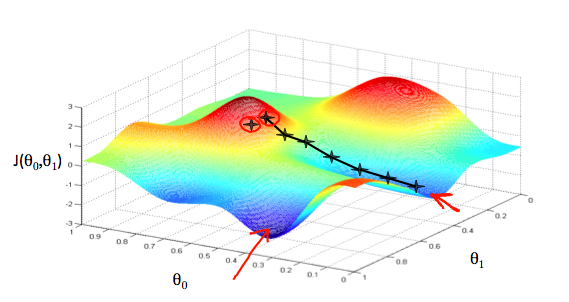
\includegraphics[width = .8\textwidth]{NotePics/2_3_1.png}

We will know that we have succeeded when our cost function is at the very bottom of the pits in our graph, i.e. when its value is the minimum. The red arrows show the minimum points in the graph.

The way we do this is by taking the derivative (the tangential line to a function) of our cost function. The slope of the tangent is the derivative at that point and it will give us a direction to move towards. We make steps down the cost function in the direction with the steepest descent. The size of each step is determined by the parameter $\alpha$, which is called the learning rate.

For example, the distance between each `star' in the graph above represents a step determined by our parameter $\alpha$. A smaller $\alpha$ would result in a smaller step and a larger $\alpha$ results in a larger step. The direction in which the step is taken is determined by the partial derivative of $J(\theta_0,\theta_1)$. Depending on where one starts on the graph, one could end up at different points. The image above shows us two different starting points that end up in two different places.

The gradient descent algorithm is:

\paragraph{repeat until convergence}

\[ \theta_j:=\theta_j - \alpha\frac{\partial J(\theta_0,\theta_1)}{\partial \theta_j} \]

where $j=0,1$ represents the feature index number.

At each iteration $j$, one should simultaneously update the parameters $\theta_1,\theta_2,...,\theta_n$. Updating a specific parameter prior to calculating another one on the $j$(th) iteration would yield to a wrong implementation.

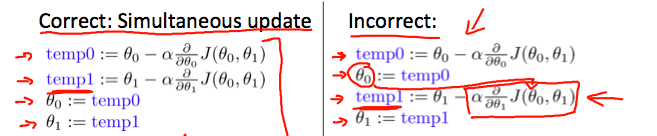
\includegraphics[width = .8\textwidth]{NotePics/2_3_2.png}

\subsubsection{Gradient Descent Intuition}

In this video we explored the scenario where we used one parameter $\theta_1$ and plotted its cost function to implement a gradient descent. Our formula for a single parameter was :

\paragraph{repeat until convergence}

\[ \theta_1:=\theta_1-\alpha\frac{dJ(\theta_1)}{d\theta_1} \]

Regardless of the slope's sign for $\frac{dJ(\theta_1)}{d\theta_1}$, $\theta_1$ eventually converges to its minimum value. The following graph shows that when the slope is negative, the value of $\theta_1$ increases and when it is positive, the value of $\theta_1$ decreases.

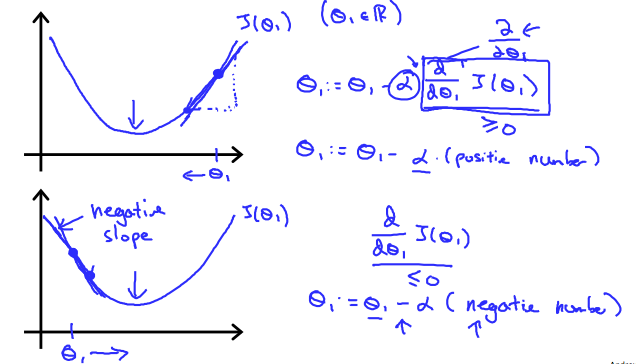
\includegraphics[width = .8\textwidth]{NotePics/2_3_1_1.png}

On a side note, we should adjust our parameter $\alpha$ to ensure that the gradient descent algorithm converges in a reasonable time. Failure to converge or too much time to obtain the minimum value imply that our step size is wrong.

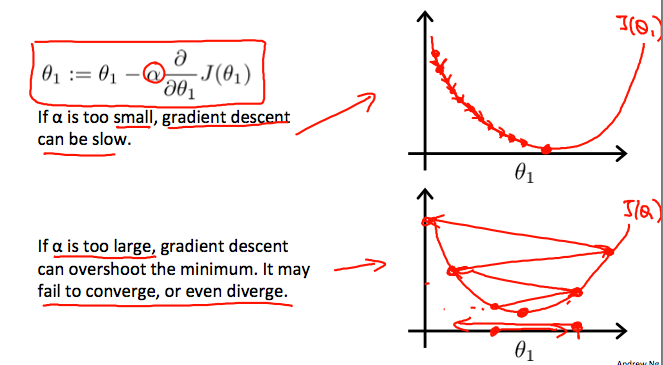
\includegraphics[width = .8\textwidth]{NotePics/2_3_1_2.png}

How does gradient descent converge with a fixed step size $\alpha$?

The intuition behind the convergence is that $\frac{dJ(\theta_1)}{d\theta_1}$ approaches 0 as we approach the bottom of our convex function. At the minimum, the derivative will always be 0 and thus we get:

\[ \theta_1:=\theta_1-a*0 \]

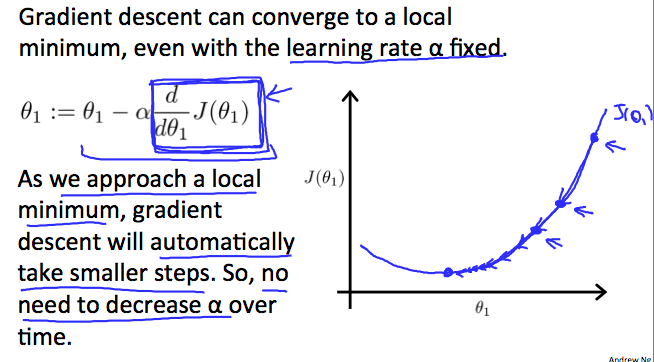
\includegraphics[width = .8\textwidth]{NotePics/2_3_1_3.png}

\subsubsection{Gradient Descent For Linear Regression}

When specifically applied to the case of linear regression, a new form of the gradient descent equation can be derived. We can substitute our actual cost function and our actual hypothesis function and modify the equation to :

repeat until convergence:

\[ \theta_0 := \theta_0-\alpha \frac{1}{m} \sum\limits_{i=1}^{m}(h_\theta(x_{i}) - y_{i}) \]
 
\[ \theta_1 := \theta_1 - \alpha \frac{1}{m} \sum\limits_{i=1}^{m}((h_\theta(x_{i}) - y_{i}) * x_{i}) \]

where $m$ is the size of the training set, $\theta_0$ a constant that will be changing simultaneously with $\theta_1$ and $x_{i}, y_{i}$ are values of the given training set (data).

Note that we have separated out the two cases for $\theta_j$ into separate equations for $\theta_0$ and $\theta_1$; and that for $\theta_1$ we are multiplying $x_{i}$ at the end due to the derivative. The following is a derivation of $\frac{\partial J(\theta)}{\partial \theta_j}$ for a single example :

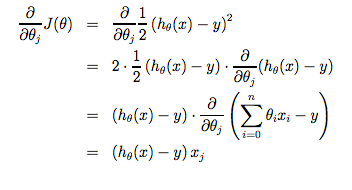
\includegraphics[width = .8\textwidth]{NotePics/2_3_2_1.png}

The point of all this is that if we start with a guess for our hypothesis and then repeatedly apply these gradient descent equations, our hypothesis will become more and more accurate.

So, this is simply gradient descent on the original cost function $J$. This method looks at every example in the entire training set on every step, and is called batch gradient descent. Note that, while gradient descent can be susceptible to local minima in general, the optimization problem we have posed here for linear regression has only one global, and no other local, optima; thus gradient descent always converges (assuming the learning rate $\alpha$ is not too large) to the global minimum. Indeed, $J$ is a convex quadratic function. Here is an example of gradient descent as it is run to minimize a quadratic function.

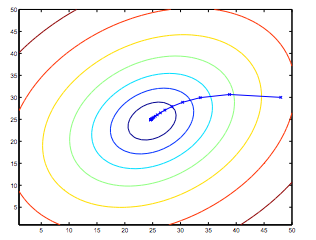
\includegraphics[width = .8\textwidth]{NotePics/2_3_2_2.png}

The ellipses shown above are the contours of a quadratic function. Also shown is the trajectory taken by gradient descent, which was initialized at (48,30). The $x$'s in the figure (joined by straight lines) mark the successive values of $\theta$ that gradient descent went through as it converged to its minimum.

\section{Lecture 3 (Optional)}

\subsection{Matrices and Vectors}

Matrices are 2-dimensional arrays:

\[ \begin{bmatrix} a&b&c\\d&e&f\\g&h&i\\j&k&l \end{bmatrix} \]

The above matrix has four rows and three columns, so it is a $4 * 3$ matrix.

A vector is a matrix with one column and many rows:

\[ \begin{bmatrix} w\\x\\y\\z \end{bmatrix} \]

So vectors are a subset of matrices. The above vector is a $4 * 1$ matrix.

\paragraph{Notation and terms}

\[ \newline \]

$A_{ij}$ refers to the element in the $i$th row and $j$th column of matrix $A$.

A vector with `$n$' rows is referred to as an `$n$'-dimensional vector.

$v_i$ refers to the element in the $i$th row of the vector.

In general, all our vectors and matrices will be 1-indexed. Note that for some programming languages, the arrays are 0-indexed.

Matrices are usually denoted by uppercase names while vectors are lowercase.

``Scalar" means that an object is a single value, not a vector or matrix.

$\mathbb{R}$ refers to the set of scalar real numbers.

$\mathbb{R}^n$ refers to the set of $n$-dimensional vectors of real numbers.

\subsection{Addition and Scalar Multiplication}

Addition and subtraction are element-wise, so you simply add or subtract each corresponding element:

\[ \begin{bmatrix} a&b\\c&d \end{bmatrix} + \begin{bmatrix} w&x\\y&z \end{bmatrix} = \begin{bmatrix} a+w&b+x\\c+y&d+z \end{bmatrix}\]

Subtracting Matrices:

\[ \begin{bmatrix} a&b\\c&d \end{bmatrix} - \begin{bmatrix} w&x\\y&z \end{bmatrix} = \begin{bmatrix} a-w&b-x\\c-y&d-z \end{bmatrix}\]

To add or subtract two matrices, their dimensions must be the same.

In scalar multiplication, we simply multiply every element by the scalar value:

\[ \begin{bmatrix} a&b\\c&d \end{bmatrix} * x = \begin{bmatrix} a*x&b*x\\c*x&d*x \end{bmatrix}\]

In scalar division, we simply divide every element by the scalar value:

\[ \begin{bmatrix} a&b\\c&d \end{bmatrix} / x = \begin{bmatrix} a/x&b/x\\c/x&d/x \end{bmatrix}\]

\subsection{Matrix-Vector Multiplication}

We map the column of the vector onto each row of the matrix, multiplying each element and summing the result.

\[ \begin{bmatrix} a&b\\c&d\\e&f \end{bmatrix} * \begin{bmatrix} x\\y \end{bmatrix} = \begin{bmatrix} a*x+b*y\\c*x+d*y\\e*x+f*y \end{bmatrix}\]

The result is a vector. The number of columns of the matrix must equal the number of rows of the vector.

An $m * n$ matrix multiplied by an $n * 1$ vector results in an $m * 1$ vector.

\subsection{Matrix-Matrix Multiplication}

We multiply two matrices by breaking it into several vector multiplications and concatenating the result.

\[ \begin{bmatrix} a&b\\c&d\\e&f \end{bmatrix} * \begin{bmatrix} w&x\\y&z \end{bmatrix} = \begin{bmatrix} a*w + b*y & a*x + b*z \\ c*w + d*y & c*x + d*z \\ e*w + f*y & e*x + f*z \end{bmatrix}\]

An $m * n$ matrix multiplied by an $n * o$ matrix results in an $m * o$ matrix. In the above example, a $3 * 2$ matrix times a $2 * 2$ matrix resulted in a $3 * 2$ matrix.

To multiply two matrices, the number of columns of the first matrix must equal the number of rows of the second matrix.

\subsection{Matrix Multiplication Properties}

\paragraph{Matrices are not commutative} $A*B\ne B*A$

\paragraph{Matrices are associative} $(A*B)*C=A*(B*C)$

The identity matrix, when multiplied by any matrix of the same dimensions, results in the original matrix. It's just like multiplying numbers by 1. The identity matrix simply has 1's on the diagonal (upper left to lower right diagonal) and 0's elsewhere.

\[ \begin{bmatrix} 1 & 0 & 0 \\ 0 & 1 & 0 \\ 0 & 0 & 1 \\ \end{bmatrix} \]

When multiplying the identity matrix after some matrix $(A*I)$, the square identity matrix's dimension should match the other matrix's columns. When multiplying the identity matrix before some other matrix $(I*A)$, the square identity matrix's dimension should match the other matrix's rows.

\subsection{Inverse and Transpose}

The inverse of a matrix $A$ is denoted $A^{-1}$. Multiplying by the inverse results in the identity matrix.

A non square matrix does not have an inverse matrix. We can compute inverses of matrices in octave with the $pinv(A)$ function and in Matlab with the $inv(A)$ function. Matrices that don't have an inverse are singular or degenerate.

The transposition of a matrix is like rotating the matrix $90^{\circ}$ in clockwise direction and then reversing it. We can compute transposition of matrices in matlab with the $transpose(A)$ function or $A'$:

\[ A = \begin{bmatrix} a & b \\ c & d \\ e & f \end{bmatrix} \]
\[ A^T = \begin{bmatrix} a & c & e \\ b & d & f \\ \end{bmatrix} \]

In other words:

$A_{ij}=A^T_{ji}$

\section{Lecture 4}

\subsection{Multiple Features}

Linear regression with multiple variables is also known as ``multivariate linear regression".

We now introduce notation for equations where we can have any number of input variables.

$x_j^{(i)}$ = value of feature $j$ in the $i^{th}$ training example

$x^{(i)}$ = the input (features) of the $i^{th}$ training example

$m$ = the number of training examples

$n$ = the number of features

The multivariable form of the hypothesis function accommodating these multiple features is as follows:

\[ h_\theta (x) = \theta_0 + \theta_1 x_1 + \theta_2 x_2 + \theta_3 x_3 + \cdots + \theta_n x_n \]

In order to develop intuition about this function, we can think about $\theta_0$ as the basic price of a house, $\theta_1$ as the price per square meter, $\theta_2$ as the price per floor, etc. $x_1$ will be the number of square meters in the house, $x_2$ the number of floors, etc.

Using the definition of matrix multiplication, our multivariable hypothesis function can be concisely represented as:

\[ h_\theta(x) = \begin{bmatrix}\theta_0 \hspace{2em} \theta_1 \hspace{2em} ... \hspace{2em} \theta_n\end{bmatrix}\begin{bmatrix}x_0 \\ x_1 \\ \vdots \\ x_n\end{bmatrix}= \theta^T x \]

This is a vectorization of our hypothesis function for one training example; see the lessons on vectorization to learn more.

\paragraph{Remark} Note that for convenience reasons in this course we assume $x_{0}^{(i)} =1$ for $(i\in { 1,\dots,m })$. This allows us to do matrix operations with $\theta$ and $x$. Hence making the two vectors $\theta$ and $x(i)$ match each other element-wise (that is, have the same number of elements: $n+1$).]

\subsection{Gradient Descent For Multiple Variables}

Gradient Descent for Multiple Variables

The gradient descent equation itself is generally the same form; we just have to repeat it for our `n' features:

\[ \theta_0 := \theta_0 - \alpha \frac{1}{m} \sum\limits_{i=1}^{m} (h_\theta(x^{(i)}) - y^{(i)}) \cdot x_0^{(i)} \]
\[ \theta_1 := \theta_1 - \alpha \frac{1}{m} \sum\limits_{i=1}^{m} (h_\theta(x^{(i)}) - y^{(i)}) \cdot x_1^{(i)} \]
\[ \theta_2 := \theta_2 - \alpha \frac{1}{m} \sum\limits_{i=1}^{m} (h_\theta(x^{(i)}) - y^{(i)}) \cdot x_2^{(i)} \]
$\cdots$

In other words:

\[ \theta_j := \theta_j - \alpha \frac{1}{m} \sum\limits_{i=1}^{m} (h_\theta(x^{(i)}) - y^{(i)}) \cdot x_j^{(i)}, \text{for } j := 0...n \]

The following image compares gradient descent with one variable to gradient descent with multiple variables:

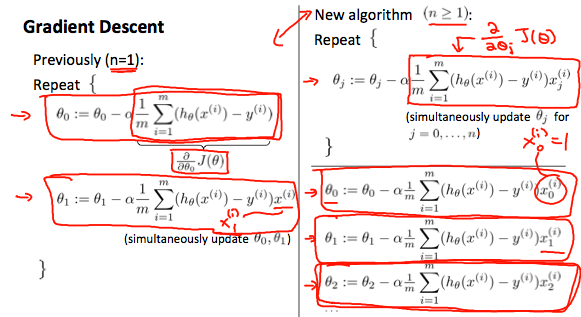
\includegraphics[width = .8\textwidth]{NotePics/4_2_1.png}

\subsubsection{Gradient Descent in Practice I - Feature Scaling}

We can speed up gradient descent by having each of our input values in roughly the same range. This is because $\theta$ will descend quickly on small ranges and slowly on large ranges, and so will oscillate inefficiently down to the optimum when the variables are very uneven.

The way to prevent this is to modify the ranges of our input variables so that they are all roughly the same. Ideally:

\[-1 \le x_{(i)} \le 1\]

or

\[ -0.5 \le x_{(i)} \le 0.5 \]

These aren't exact requirements; we are only trying to speed things up. The goal is to get all input variables into roughly one of these ranges, give or take a few.

Two techniques to help with this are feature scaling and mean normalization. Feature scaling involves dividing the input values by the range (i.e. the maximum value minus the minimum value) of the input variable, resulting in a new range of just 1. Mean normalization involves subtracting the average value for an input variable from the values for that input variable resulting in a new average value for the input variable of just zero. To implement both of these techniques, adjust your input values as shown in this formula:

\[ x_i := \dfrac{x_i - \mu_i}{s_i} \]

Where $\mu_i$ is the average of all the values for feature $(i)$ and $s_i$ is the range of values $(max - min)$, or $s_i$ is the standard deviation.

Note that dividing by the range, or dividing by the standard deviation, give different results. The quizzes in this course use range - the programming exercises use standard deviation.

For example, if $x_i$ represents housing prices with a range of 100 to 2000 and a mean value of 1000, then, 

\[ x_i := \dfrac{price-1000}{1900} \]

\subsubsection{Gradient Descent in Practice II - Learning Rate}

\paragraph{Debugging gradient descent} Make a plot with number of iterations on the $x$-axis. Now plot the cost function, $J(\theta)$ over the number of iterations of gradient descent. If $J(\theta)$ ever increases, then you probably need to decrease $\alpha$.

\paragraph{Automatic convergence test} Declare convergence if $J(\theta)$ decreases by less than $E$ in one iteration, where $E$ is some small value such as $10^{-3}$. However in practice it's difficult to choose this threshold value.

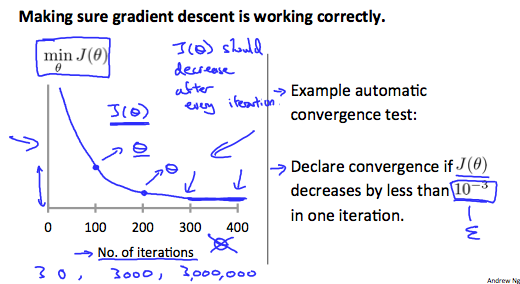
\includegraphics[width = .8\textwidth]{NotePics/4_2_2_1.png}

It has been proven that if learning rate $\alpha$ is sufficiently small, then $J(\theta)$ will decrease on every iteration.

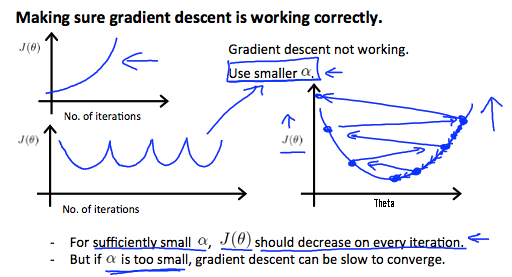
\includegraphics[width = .8\textwidth]{NotePics/4_2_2_2.png}

To summarize:

If $\alpha$ is too small: slow convergence.

If $\alpha$ is too large: may not decrease on every iteration and thus may not converge.

\subsection{Features and Polynomial Regression}

We can improve our features and the form of our hypothesis function in a couple different ways.

We can combine multiple features into one. For example, we can combine $x_1$ and $x_2$ into a new feature $x_3$ by taking $x_1*x_2$.

\paragraph{Polynomial Regression}

Our hypothesis function need not be linear (a straight line) if that does not fit the data well.

We can change the behavior or curve of our hypothesis function by making it a quadratic, cubic or square root function (or any other form).

For example, if our hypothesis function is $h_\theta(x) = \theta_0 + \theta_1 x_1$ then we can create additional features based on $x_1$, to get the quadratic function $h_\theta(x) = \theta_0 + \theta_1 x_1 + \theta_2 x_1^2$ or the cubic function $h_\theta(x) = \theta_0 + \theta_1 x_1 + \theta_2 x_1^2 + \theta_3 x_1^3$

In the cubic version, we have created new features $x_2$ and $x_3$ where $x_2=x_1^2$ and $x_3=x_1^3$.

To make it a square root function, we could do: $h_\theta(x) = \theta_0 + \theta_1 x_1 + \theta_2 \sqrt{x_1}$.

One important thing to keep in mind is, if you choose your features this way then feature scaling becomes very important.

eg. if $x_1$ has range 1 - 1000 then range of $x_1^2$ becomes 1 - 1000000 and that of $x_1^3$ becomes 1 - 1000000000.

\subsection{Normal Equation}

Gradient descent gives one way of minimizing $J$. Let's discuss a second way of doing so, this time performing the minimization explicitly and without resorting to an iterative algorithm. In the ``Normal Equation" method, we will minimize $J$ by explicitly taking its derivatives with respect to the $\theta_j$'s, and setting them to zero. This allows us to find the optimum theta without iteration. The normal equation formula is given below:

\[ \theta = (X^T X)^{-1}X^T y \]

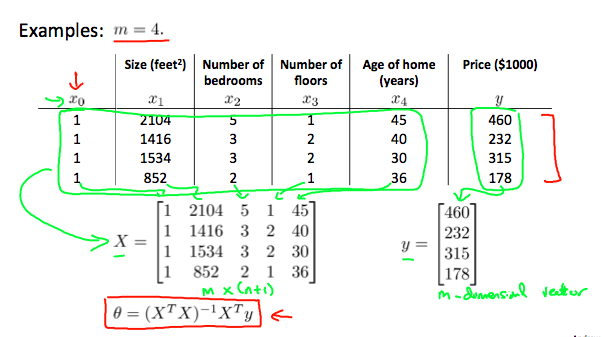
\includegraphics[width = .8\textwidth]{NotePics/4_4_1.png}

There is no need to do feature scaling with the normal equation.

The following is a comparison of gradient descent and the normal equation:

\begin{tabular}{|c|c|}
 \hline
Gradient Descent & Normal Equation\\
 \hline
Need to choose alpha & No need to choose alpha \\
 \hline
Needs many iterations & No need to iterate \\
 \hline
$\mathcal{O}{(kn^2)}$ & $\mathcal{O}{(n^3)}$, need to calculate inverse of $X^T X$ \\
 \hline
Works well when $n$ is large & Slow if $n$ is very large \\
 \hline
\end{tabular}

With the normal equation, computing the inversion has complexity $\mathcal{O}(n^3)$. So if we have a very large number of features, the normal equation will be slow. In practice, when $n$ exceeds 10,000 it might be a good time to go from a normal solution to an iterative process.

\subsubsection{Normal Equation Noninvertibility (Optional)}

When implementing the normal equation in octave we want to use the `$pinv$' function rather than `$inv$.' The `$pinv$' function will give you a value of $\theta$ even if $X^T X$ is not invertible.

If $X^T X$ is noninvertible, the common causes might be having:

\paragraph{Redundant features} Where two features are very closely related (i.e. they are linearly dependent)

\paragraph{Too many features (e.g. $m \le n$)} In this case, delete some features or use ``regularization" (to be explained in a later lesson).

Solutions to the above problems include deleting a feature that is linearly dependent with another or deleting one or more features when there are too many features.

\end{document}
